% Chapter 3 -- Statistics for Noisy Returns
% Requires: amsmath, amssymb, booktabs, array, tabularx, graphicx, tcolorbox (breakable, skins), hyperref or url.
% Defines the callout box only if the preamble has not.
\providecolor{fenavy}{HTML}{1B2A6B}
\providecolor{feshade}{HTML}{F3F5FA}
\makeatletter
\@ifundefined{callout}{%
  \newtcolorbox{callout}{breakable, enhanced,
    colback=white, colframe=gray!70, boxrule=0.5pt, arc=1mm,
    borderline west={2.5pt}{0pt}{gray!70},
    left=8pt, right=8pt, top=4pt, bottom=4pt}%
}{}
\makeatother

\chapter{Statistics for Noisy Returns}
\label{ch:03}

Part II of the book turns the lessons of Part I into tools. It begins with the most basic tool of all: the t-statistic.

Almost every claim in quantitative finance ends in a number like ``$t = 2.4$.'' That number comes from formulas taught in introductory statistics, which assume that observations are independent, that their spread is constant, and that their distribution is roughly normal. Financial returns satisfy none of these assumptions exactly. Their tails are fat, their volatility comes in clusters, and some of the most popular research designs build in strong dependence between observations. The good news is that each departure has a well-tested remedy, and choosing the right one is a skill you can learn in a single chapter.

The claim on trial in this chapter is the one every researcher relies on: \textbf{with the right standard errors, regression statistics are reliable for financial returns.} The lab tests it in two settings: one where the usual formulas already work well, and one where the choice of standard error decides whether a ``significant'' result is real.

By the end of the chapter you will be able to:

\begin{itemize}
  \item summarize a return distribution by its mean, variance, skewness, kurtosis and autocorrelation;
  \item run and interpret a linear regression, including its slope, intercept and $R^2$, and explain what heteroskedasticity and serial correlation do to its standard errors;
  \item explain the CAPM and the Fama--French three-factor model, and interpret beta and alpha;
  \item describe the stylized facts of financial returns: fat tails, volatility clustering, weak autocorrelation and asymmetry;
  \item choose standard errors that remain valid when those features are present: White, Newey--West and clustered errors;
  \item explain why overlapping long-horizon regressions mislead, and how to correct them;
  \item test a factor model with alphas, the GRS test and Fama--MacBeth regressions;
  \item use the bootstrap to measure uncertainty without relying on normality;
  \item separate statistical significance from economic significance.
\end{itemize}

In the lab you will measure these features on nearly a century of real data, compute the alphas of 25 classic portfolios four different ways, and run a controlled experiment that shows how often overlapping regressions find predictability that is not there.

\section{Foundations: distributions, regression and factor models}
\label{sec:03-foundations}

\textbf{Describing a distribution.} Four numbers, called \textbf{moments}, summarize a return distribution.

\begin{itemize}
  \item The \textbf{mean} is its center: the average return.
  \item The \textbf{variance}, or its square root the standard deviation, measures spread: how far returns typically fall from the mean.
  \item \textbf{Skewness} measures asymmetry. It is negative when large losses are more likely than large gains of the same size, as for most stock indexes.
  \item \textbf{Kurtosis} measures how heavy the tails are. A normal distribution has kurtosis 3; values above 3 indicate \textbf{fat tails}, meaning extreme returns occur more often than a normal distribution predicts.
\end{itemize}

Figure~\ref{fig:03-moments} shows what each of the four moments changes, by comparing the normal distribution with one that differs in that moment alone.

\begin{figure}[htbp]
\centering
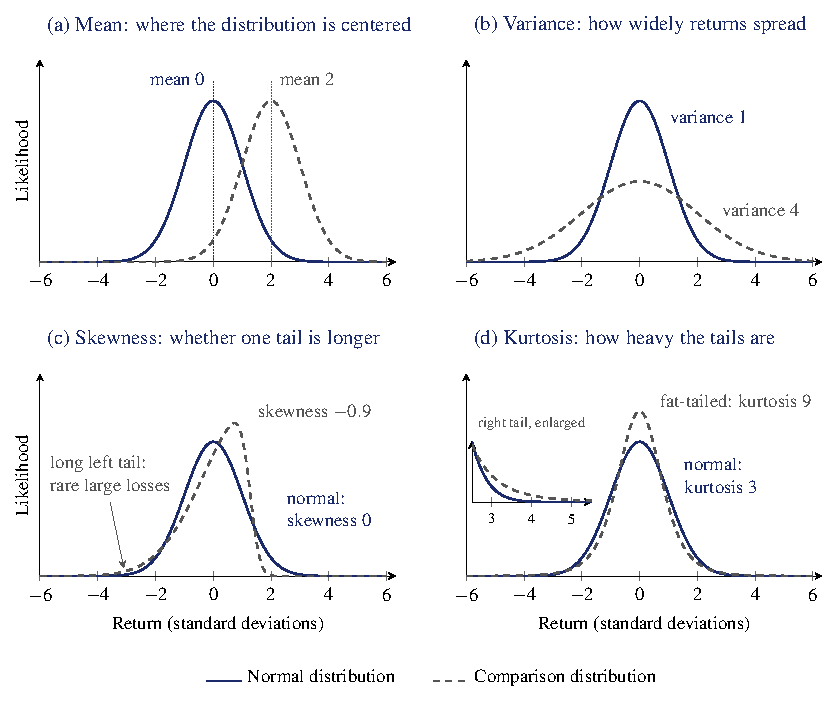
\includegraphics[width=0.95\linewidth]{images/fig03-0-moments.pdf}
\caption{The four moments of a distribution. Each panel compares the standard normal distribution (solid) with one that differs in a single respect. (a)~The mean sets the center. (b)~The variance sets the spread. (c)~Negative skewness lengthens the left tail, so large losses are more likely than large gains of the same size. (d)~Higher kurtosis puts more weight in the tails: the normal distribution has kurtosis 3, the fat-tailed one shown has kurtosis 9. Panels (c) and (d) keep the mean and variance of the normal distribution.}
\label{fig:03-moments}
\end{figure}

A fifth measure describes behavior over time. \textbf{Autocorrelation} is the correlation of a series with its own past values: the first-order autocorrelation compares each month with the month before. A return series with zero autocorrelation cannot be predicted from its own history.

\textbf{Linear regression.} A regression describes how one variable, $y$, moves with another, $x$. Ordinary least squares (OLS) fits
\begin{equation}
  y_t = \alpha + \beta x_t + \varepsilon_t
  \label{eq:03-ols}
\end{equation}
by choosing the intercept $\alpha$ and slope $\beta$ that make the \textbf{residuals} $\varepsilon_t$, the gaps between the actual values and the fitted line, as small as possible in the sense of their sum of squares. The slope $\beta$ measures how much $y$ moves when $x$ moves by one unit. The \textbf{R-squared}, $R^2$, is the share of the variance of $y$ that the regression explains, from 0 (none) to 1 (all).

Each estimate comes with a standard error, and the usual formula for it assumes that the residuals are independent of one another and have the same variance throughout. Two departures from these assumptions are common in finance:

\begin{itemize}
  \item \textbf{Heteroskedasticity}: the variance of the residuals changes over time or across observations, for example rising in a crisis.
  \item \textbf{Serial correlation}: residuals are correlated with their own past values, so one large error tends to be followed by another.
\end{itemize}

When either is present, the coefficient estimates usually remain reasonable, but the usual standard errors are wrong, and the corrections developed in this chapter are needed.

\textbf{The capital asset pricing model.} The CAPM of Sharpe (1964), Lintner (1965) and Mossin (1966) says that an asset's expected excess return is proportional to its \textbf{beta}, its sensitivity to the market:
\begin{equation}
  E[R_i] - r_f = \beta_i \left(E[R_m] - r_f\right), \qquad \beta_i = \frac{\operatorname{Cov}(R_i, R_m)}{\operatorname{Var}(R_m)}
  \label{eq:03-capm}
\end{equation}
Here $\operatorname{Cov}$ is the covariance, which measures how two returns move together, and $\operatorname{Var}$ the variance. A stock with a beta of 1.5 tends to rise 1.5\% when the market rises 1\%. Only market risk is rewarded, because other risk can be removed by holding many stocks, which is called \textbf{diversification}. Empirically, the model is tested with a time-series regression of an asset's excess return on the market's excess return, as in Section~\ref{sec:01-foundations}. The intercept, \textbf{alpha}, is the average return the CAPM fails to explain; the model predicts that alpha is zero for every asset. Figure~\ref{fig:03-alpha} shows the two numbers on a scatter plot.

\begin{figure}[htbp]
\centering
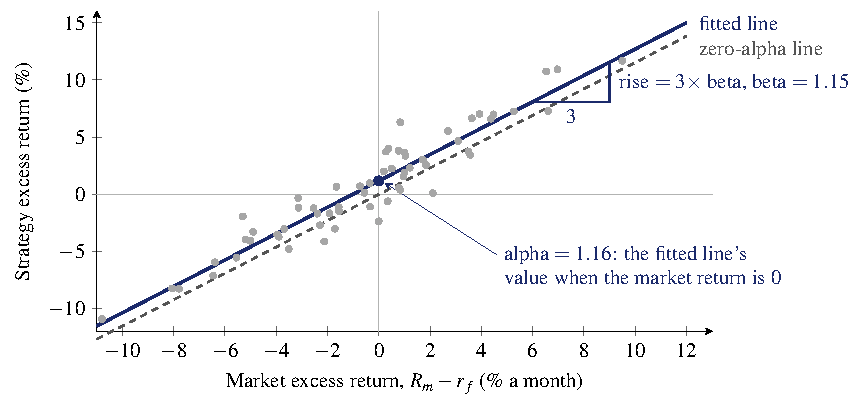
\includegraphics[width=0.85\linewidth]{images/fig03-1-regression-alpha.pdf}
\caption{Beta and alpha in a regression of a strategy's monthly excess returns on the market's. Beta is the slope of the fitted line; alpha is its height where the market's excess return is zero, the gap between the fitted line and a line with the same slope through the origin. Simulated data, with an alpha larger than any real strategy's so that it is visible.}
\label{fig:03-alpha}
\end{figure}

\textbf{Multifactor models.} The CAPM fits the data poorly: small stocks and value stocks have earned more than their betas imply (Chapter 8). \textbf{Factor models} add further sources of risk, called factors. The Fama--French three-factor model adds two:

\begin{itemize}
  \item SMB (small minus big): the return of small stocks over large ones;
  \item HML (high minus low): the return of value stocks, with high book-to-market ratios, over growth stocks, with low ones.
\end{itemize}

The model is
\begin{equation}
  R_i - r_f = \alpha_i + b_i(R_m - r_f) + s_i\,\mathrm{SMB} + h_i\,\mathrm{HML} + \varepsilon_i
  \label{eq:03-ff3}
\end{equation}
where $b_i$, $s_i$ and $h_i$ measure the asset's exposure to each factor. The factors are themselves \textbf{long--short} portfolio returns: each buys one group of stocks and sells the other short, so it costs roughly nothing to set up. A strategy's alpha relative to a factor model measures what it earns beyond its exposures to those factors.

\textbf{Testing many alphas at once.} If a model is correct, the alphas of all assets should be jointly zero. The GRS test (Gibbons, Ross and Shanken 1989) tests this for a set of portfolios. The \textbf{Fama--MacBeth} procedure (Fama and MacBeth 1973) asks a related question: is a characteristic or beta rewarded across assets? Each month it regresses returns across assets on their betas, then averages the monthly slopes over time. Sections~\ref{sec:03-grs} and~\ref{sec:03-fmb} develop both.

\textbf{Worked example.} A fund's monthly excess returns are regressed on the market's. The estimated beta is 1.1 and alpha is 0.2\% a month with a standard error of 0.15\%. The alpha's t-statistic is $0.2/0.15 = 1.33$: the fund may have skill, but the data cannot distinguish its alpha from zero.


\section{Stylized facts of financial returns}
\label{sec:03-facts}

The textbook standard error rests on three assumptions: observations are
independent, their variance is constant, and their distribution is roughly
normal. Real returns depart from all three in consistent ways. This section
describes the four departures that matter most, and shows which assumption each
one breaks.

Decades of research have documented these features across markets, assets and
periods. Cont (2001) collected them as ``stylized facts,'' patterns found so
consistently that any model of returns must reproduce them:

\begin{enumerate}
  \item \textbf{Fat tails.} Extreme returns happen far more often than a normal distribution predicts (Figure~\ref{fig:03-tails}). Mandelbrot (1963) and Fama (1965) documented this in the 1960s. On October 19, 1987, the U.S. market fell by more than 20\% in a day, a move a normal distribution fitted to daily data would treat as essentially impossible. For daily stock index returns, kurtosis is typically far higher than the normal distribution's 3.
  \item \textbf{Volatility clustering.} Large moves tend to follow large moves, of either sign, and calm periods follow calm periods. Returns themselves show little autocorrelation, but their absolute values and squares are strongly and persistently autocorrelated. Chapter 11 builds forecasting models on this feature.
  \item \textbf{Weak autocorrelation in returns.} Daily and monthly index returns show only small autocorrelations, consistent with Section~\ref{sec:01-efficient-markets}. Some portfolios, especially of small stocks, show more, partly because their prices are \textbf{stale}: some stocks do not trade every day, so their last recorded price lags the news.
  \item \textbf{Asymmetry.} Large falls are more common than large rises of the same size, and volatility tends to rise after falls. The rise in volatility after a fall is called the \textbf{leverage effect}, because a falling share price raises a company's debt relative to its equity.
\end{enumerate}

\begin{figure}[htbp]
\centering
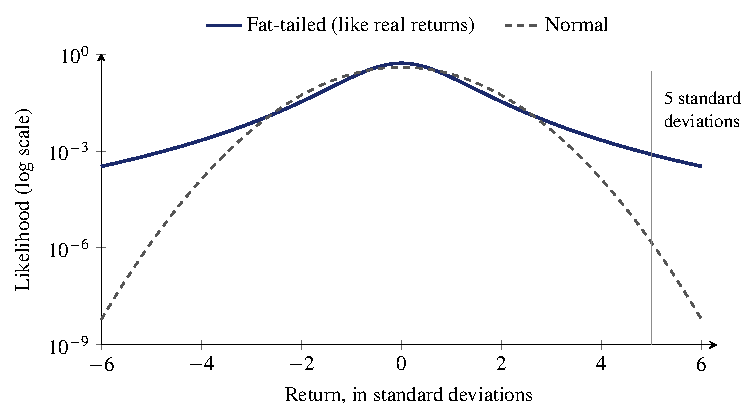
\includegraphics[width=0.85\linewidth]{images/fig03-2-fat-tails.pdf}
\caption{Fat tails. Both curves have the same mean and standard deviation. On a log scale the difference in the tails becomes visible: a daily move of five standard deviations in either direction occurs about once in 7,000 years under the normal distribution, but about once every two years under the fat-tailed distribution shown, a Student-$t$ distribution with four degrees of freedom, which is a common model for daily returns.}
\label{fig:03-tails}
\end{figure}

\textbf{Why this matters for statistics.} None of these features biases the
regression estimates themselves, which usually remain right on average. What
they damage is the stated precision of those estimates, and with it every
t-statistic and \textbf{p-value}, the probability of a result at least this
extreme if the true effect were zero (Chapter 4). Each feature breaks a
different assumption, and the rest of the chapter deals with each in turn:

\begin{center}
\small
\begin{tabularx}{0.95\linewidth}{@{}>{\raggedright\arraybackslash}p{0.26\linewidth}>{\raggedright\arraybackslash}X>{\raggedright\arraybackslash}p{0.33\linewidth}@{}}
\toprule
Feature & Assumption it breaks & Remedy \\
\midrule
Volatility clustering & Constant variance & White or Newey--West standard errors (Section~\ref{sec:03-se}) \\
Autocorrelation and stale prices & Independence & Newey--West standard errors (Section~\ref{sec:03-se}) \\
Overlapping research designs & Independence, severely & Newey--West with enough lags, or Hodrick (1992) (Section~\ref{sec:03-overlap}) \\
Fat tails & Normality, so small-sample p-values are off & The bootstrap (Section~\ref{sec:03-bootstrap}) \\
\bottomrule
\end{tabularx}
\end{center}

\section{Choosing the right standard error}
\label{sec:03-se}

The estimates from a regression are usually reliable even when returns violate
the textbook assumptions. Their standard errors are not. The right standard
error is the one that allows for the dependence your data actually have: errors
whose variance changes over time, errors that move together over time, or
errors that move together across firms.

Consider the regression that appears throughout this book, a time-series
regression of a portfolio's excess return on one or more factors:
\begin{equation}
  r_t = \alpha + \beta' f_t + \varepsilon_t
  \label{eq:03-ts}
\end{equation}
where $f_t$ is the list of factor returns in month $t$ and $\beta'$ the list of
the portfolio's exposures to them. The classical standard error assumes that
the errors $\varepsilon_t$ are independent and equally variable. Three
alternatives relax these assumptions one step at a time:

\begin{itemize}
  \item \textbf{White (1980)} allows the variance of the errors to change over
  time, as it does when volatility clusters.
  \item \textbf{Newey--West (1987)} also allows errors up to $L$ periods apart
  to be correlated. It is called a \textbf{HAC} estimator, for
  \emph{heteroskedasticity and autocorrelation consistent}.
  \item \textbf{Clustered} standard errors allow errors within a group, such as
  all firms in the same month, to be correlated (Petersen 2009).
\end{itemize}

\textbf{Which to use.} Match the standard error to the data:

\begin{center}
\small
\begin{tabularx}{0.95\linewidth}{@{}>{\raggedright\arraybackslash}p{0.34\linewidth}>{\raggedright\arraybackslash}p{0.28\linewidth}>{\raggedright\arraybackslash}X@{}}
\toprule
Your data & Use & Why \\
\midrule
Monthly returns, no overlap & White, or Newey--West with a few lags & Volatility changes, but errors are close to independent \\
Errors correlated over time (daily data, stale prices, persistent predictors) & Newey--West & Nearby errors move together \\
Overlapping $k$-period returns & Newey--West with at least $k-1$ lags, or Hodrick (1992) & The overlap builds in correlation $k-1$ periods long (Section~\ref{sec:03-overlap}) \\
Many firms over many periods & Clustered by firm and by time & Errors move together within a month and within a firm \\
\bottomrule
\end{tabularx}
\end{center}

When in doubt, report Newey--West. If the data have no dependence, it gives
almost the same answer as the classical formula, so little is lost; if they
do, it protects you from false confidence. Part B of the lab shows the first
case and Part C the second.

\textbf{Choosing the lag.} Newey--West needs one setting, the number of lags
$L$. A common rule of thumb is $L = \lfloor 4(T/100)^{2/9} \rfloor$, where
$\lfloor\cdot\rfloor$ means rounding down: 50 years of monthly data, $T = 600$,
gives $L = 5$. When the design creates dependence of a known length, such as
$k$-month overlapping returns, use at least $k - 1$ lags.

\textbf{How Newey--West works.} For readers who want the detail: every
standard error rests on an estimate of how much the regression's errors vary
and move together. Newey--West estimates it as
\begin{equation}
  \hat S = \sum_t x_t x_t' \hat\varepsilon_t^2 + \sum_{\ell=1}^{L} \left(1 - \frac{\ell}{L+1}\right) \sum_t \left(x_t \hat\varepsilon_t \hat\varepsilon_{t-\ell} x_{t-\ell}' + x_{t-\ell} \hat\varepsilon_{t-\ell} \hat\varepsilon_t x_t'\right)
  \label{eq:03-nw}
\end{equation}
where $x_t$ holds the regressors in period $t$. The first sum is White's
estimator, which lets each period have its own variance. The second adds the
correlations between errors up to $L$ periods apart, with weights that shrink
as the gap $\ell$ grows.

\section{Overlapping observations: less data than it seems}
\label{sec:03-overlap}

Long-horizon regressions can look far stronger than they are. When each
observation's return overlaps the next, a sample that seems to hold hundreds of
observations holds only a handful of independent ones, and the classical
t-statistic and $R^2$ overstate the evidence accordingly.

\textbf{The design.} A popular design in return-prediction research regresses
returns over a long horizon, such as the next five years, on a predictor
measured today, such as the dividend yield:
\begin{equation}
  r_{t+1} + r_{t+2} + \dots + r_{t+k} = a + b\,x_t + u_{t+k}
  \label{eq:03-longhorizon}
\end{equation}

\textbf{The problem: counting observations.} With monthly data and $k = 60$,
each observation's dependent variable shares 59 of its 60 months with the next
observation's (Figure~\ref{fig:03-overlap}). The regression appears to have
hundreds of observations but contains roughly $T/k$ independent ones. Fifty
years of monthly data, $T = 600$, give only $600/60 = 10$ independent five-year
returns.

\begin{figure}[htbp]
\centering
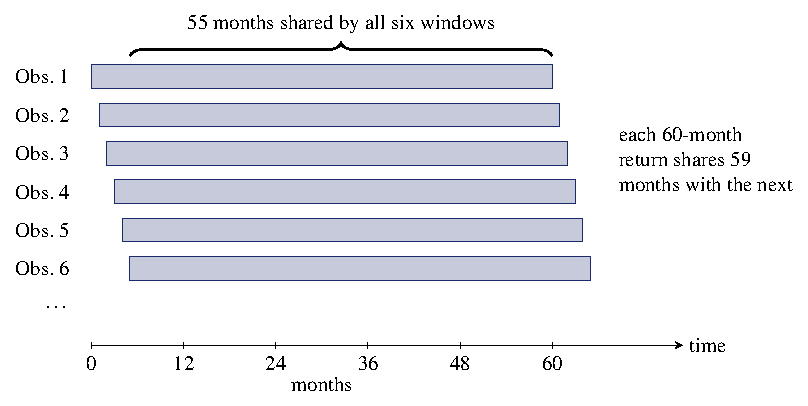
\includegraphics[width=0.85\linewidth]{images/fig03-3-overlap.pdf}
\caption{Overlapping observations. Each observation in a regression of five-year returns covers 60 months, and each starts one month after the last. Consecutive observations share 59 of their 60 months, so they carry almost the same information.}
\label{fig:03-overlap}
\end{figure}

\textbf{Two consequences.}

\begin{enumerate}
  \item \textbf{Standard errors that are far too small.} The errors $u$ are strongly autocorrelated by construction, up to lag $k - 1$. Classical standard errors ignore this and can be several times too small. Hansen and Hodrick (1980) and Newey--West correct for the overlap, but in samples of typical length they still reject a true null hypothesis too often. A test's \textbf{size} is the rate at which it does so; a well-behaved 5\% test has a size of 5\%. Hodrick (1992) proposed an alternative that avoids overlapping errors and has more reliable size.
  \item \textbf{Biased slopes from persistent predictors.} A variable is \textbf{persistent} when it moves slowly, so that this month's value is close to last month's. The dividend yield has a monthly autocorrelation close to 1. Stambaugh (1999) showed that when the predictor's surprises are correlated with return surprises, as they are for valuation ratios, the estimated slope is biased in finite samples. Valkanov (2003) showed that with overlapping horizons and persistent predictors, t-statistics do not even converge to the normal distribution, so the usual critical values are wrong.
\end{enumerate}

\textbf{A rising $R^2$ is not evidence.} $R^2$ tends to rise with the horizon
even when there is no predictability at all. Long-horizon regressions
mechanically add up the same short-horizon information, so a rising $R^2$ does
not by itself show that returns become more predictable in the long run.

\textbf{What to do.} Before trusting a long-horizon result:

\begin{itemize}
  \item count the independent observations, roughly $T/k$, before reading any t-statistic;
  \item use Newey--West with at least $k-1$ lags, or better, Hodrick's (1992) method;
  \item check the one-period regression first: a long-horizon result adds little if the one-period evidence is weak;
  \item treat persistent predictors, such as valuation ratios, with extra caution.
\end{itemize}

\begin{callout}
\textbf{What Failed: the long-horizon evidence.} In the late 1980s and 1990s, regressions of multi-year returns on dividend yields reported $R^2$ values of 30\% or more and large t-statistics, and were widely read as strong evidence that stock returns are predictable over long horizons. Later work showed how much of that strength came from the design. Valkanov (2003) and Boudoukh, Richardson and Whitelaw (2008) argued that, once overlap and persistence are accounted for, long-horizon regressions add little beyond what the one-period regression already shows, and that one-period evidence is weak. Chapter 7 tests return predictability directly; the lab in this chapter shows the statistical mechanism.
\end{callout}

\section{Testing factor models: are all the alphas zero?}
\label{sec:03-grs}

A factor model is judged by what it leaves unexplained. If the model is right,
every portfolio's alpha is zero. The right way to check is to test all the
alphas together, because testing them one at a time is almost certain to find
some that look significant by chance.

\textbf{What is being tested.} A factor model says that a portfolio's expected
excess return is explained by its exposures to a few common factors. In the
CAPM the only factor is the market; in the Fama--French (1993) three-factor
model the market is joined by size (SMB) and value (HML). If the model is
right, every portfolio's alpha in the time-series regression of
Equation~\eqref{eq:03-ts} is zero.

\textbf{Why one alpha at a time is not enough.} The alpha's t-statistic tests
whether a single portfolio is priced correctly. With 25 portfolios, about one
would show $|t| > 2$ by chance even if the model were perfect: the
multiple-testing problem from Chapter 1 in a new setting.

\textbf{All alphas at once: the GRS test.} Gibbons, Ross and Shanken (1989)
derived a joint test that all $N$ alphas are zero. With $T$ months, $N$
portfolios and $L$ factors, the GRS statistic is
\begin{equation}
  \mathrm{GRS} = \frac{T}{N}\cdot\frac{T-N-L}{T-L-1}\cdot\frac{\hat\alpha'\hat\Sigma^{-1}\hat\alpha}{1+\bar f'\hat\Omega^{-1}\bar f}
  \label{eq:03-grs}
\end{equation}
where $\hat\alpha$ is the list of estimated alphas, $\hat\Sigma$ the covariance
matrix of the regression residuals, $\bar f$ the average factor returns and
$\hat\Omega$ their covariance matrix. Under normal, independent errors it
follows an \textbf{F distribution} with $N$ and $T - N - L$ \textbf{degrees of
freedom}, the standard distribution for tests of several restrictions at once,
so its p-value can be read from a table. The statistic has an intuitive
reading: it measures how much the best Sharpe ratio achievable from the
portfolios and factors together exceeds the best Sharpe ratio from the factors
alone. If the portfolios add nothing to the factors, the model is complete.

\textbf{What GRS can and cannot show.} A small GRS statistic means the model
leaves no detectable pattern in alphas; a large one means it misprices at least
some portfolios. It does not say which, nor whether the mispricing is
economically large. GRS also relies on normal, independent errors, so with fat
tails and clustering its p-values are approximate. Fama and French (1993) found
that their three factors absorbed most of the alpha patterns that the CAPM left
in size and book-to-market portfolios, though the joint test still rejected the
model, and the smallest growth stocks remained a persistent problem.

\textbf{How to use it.} Report the GRS statistic and its p-value together with
the alphas themselves, in percent per year: the test says whether the model
fails, and the alphas show where and by how much. With fat-tailed returns,
check the p-value with a bootstrap (Section~\ref{sec:03-bootstrap}).

\section{Fama--MacBeth regressions: is a risk rewarded?}
\label{sec:03-fmb}

The GRS test asks whether a model's alphas are zero. Fama--MacBeth regressions
ask a different question: do assets with more exposure to a factor earn more on
average, and how much more per unit of exposure? That amount is the factor's
\textbf{risk premium}, $\lambda$, and the Fama--MacBeth method estimates it with
a standard error that allows for correlation across assets.

\textbf{The procedure.} The regressions are \textbf{cross-sectional}: they
compare many assets at the same moment. Fama and MacBeth (1973) introduced a
two-step procedure that remains the standard:

\begin{enumerate}
  \item \textbf{Estimate exposures.} For each of $N$ portfolios, regress its excess returns on the factors over time to estimate its betas.
  \item \textbf{Run a cross-section each month.} For each month $t$, regress the $N$ portfolio returns on their betas. Keep the slopes $\hat\lambda_t$, one set per month.
\end{enumerate}

The risk-premium estimate is the average of the monthly slopes, and its standard
error comes from their variation over time:
\begin{equation}
  \hat\lambda = \frac{1}{T}\sum_{t=1}^{T}\hat\lambda_t, \qquad \mathrm{se}(\hat\lambda) = \frac{s(\hat\lambda_t)}{\sqrt{T}}
  \label{eq:03-fmb}
\end{equation}
where $s(\hat\lambda_t)$ is the standard deviation of the monthly slopes. This
is why the method handles correlation across portfolios automatically: a
market-wide shock in one month moves that month's $\hat\lambda_t$, and its
effect shows up in the time-series variation of the slopes.

\textbf{Two cautions.} First, the betas in step 2 are estimates, not true
values. Using a noisy estimate in place of the true variable is an
\textbf{errors-in-variables} problem, and it makes the second-step standard
errors too small. Shanken (1992) derived a correction that inflates the
Fama--MacBeth variance by a factor that depends on the factors' Sharpe ratios.
Second, Fama--MacBeth standard errors assume the monthly slopes are independent
over time; if they are autocorrelated, apply Newey--West to the series of
slopes.

\textbf{How to use it.} Report Shanken-corrected t-statistics, and compare each
estimated premium with the factor's own average return: if the model is right,
the two should match. A classic finding the lab replicates is that the
estimated price of market beta is often far below the market's average excess
return, and sometimes close to zero, with a positive intercept. In other words,
high-beta portfolios have not earned as much more as the CAPM predicts.
Chapter 12 returns to this as the low-risk anomaly.

\section{The bootstrap: uncertainty without a formula}
\label{sec:03-bootstrap}

Every standard error so far comes from a formula, and every formula rests on
assumptions. The \textbf{bootstrap}, introduced by Efron (1979), avoids the
formula: it measures uncertainty by recomputing a statistic on many resampled
versions of the data, so fat tails and other features of the sample are carried
into the answer automatically. For returns, one rule matters above all:
resample blocks of consecutive observations, not single months.

\textbf{The recipe.}

\begin{enumerate}
  \item Draw $T$ observations at random from the sample, \textbf{with replacement}, so that some observations appear more than once and others not at all.
  \item Recompute the statistic, such as a Sharpe ratio or an alpha, on this new sample.
  \item Repeat a few thousand times.
  \item Use the spread of the recomputed values as the standard error or confidence interval.
\end{enumerate}

\textbf{Resample blocks, not points.} Drawing individual months at random
destroys any dependence over time, including volatility clustering. For time
series, the bootstrap must resample blocks of consecutive observations:

\begin{itemize}
  \item The \textbf{moving-block bootstrap} draws blocks of fixed length $b$.
  \item The \textbf{stationary bootstrap} of Politis and Romano (1994) draws blocks of random length, with mean length $b$. This keeps the resampled series \textbf{stationary}, meaning its statistical properties do not depend on the date. It is the default in this book.
\end{itemize}

When a regression involves several series, such as a portfolio and the factors,
resample entire rows together so that the relationships between them are
preserved.

\textbf{When to use it.} Use the bootstrap when no reliable formula exists or
its assumptions are doubtful: confidence intervals for Sharpe ratios and alphas
with fat-tailed returns, a check on the GRS p-value, or tests of whether the
best performers in a group beat what luck would produce. Kosowski, Timmermann,
Wermers and White (2006) and Fama and French (2010) used it to ask whether top
mutual fund managers have genuine skill, an empirical version of the random
strategies in Lab 1.

\textbf{What it cannot do.} The bootstrap reproduces the sample, so it cannot
create information the sample lacks. With a short sample or a rare event, such
as a single crash, the resampled data will reflect that event's frequency in
the sample and nothing more.

\section{Statistical versus economic significance}
\label{sec:03-economic}

A result can be statistically significant and still not worth acting on, and a
result worth acting on can fail to be significant. Before believing or
dismissing any finding, ask two separate questions: is it real, and is it
large enough to matter?

A t-statistic answers only the first: how surprising would this estimate be if
the true effect were zero? An effect is \textbf{statistically significant} if it
is unlikely to be due to chance, and \textbf{economically significant} if it is
large enough to change what an investor would do. The two can diverge in both
directions:

\begin{center}
\small
\begin{tabularx}{0.9\linewidth}{@{}>{\raggedright\arraybackslash}p{0.20\linewidth}>{\raggedright\arraybackslash}X>{\raggedright\arraybackslash}X@{}}
\toprule
 & Economically small & Economically large \\
\midrule
\textbf{Statistically significant} & A tiny alpha measured precisely, such as 0.5\% a year on a low-risk, high-turnover strategy whose costs exceed it & The claims worth acting on, if they survive the rest of the book's tests \\
\textbf{Not significant} & Nothing to see & A large alpha measured imprecisely, such as 6\% a year over a short, volatile record (Section~\ref{sec:01-signal-noise}) \\
\bottomrule
\end{tabularx}
\end{center}

Three habits keep the two apart:

\begin{enumerate}
  \item \textbf{Always report the size of the effect in units that matter}: percent per year, dollars, or a change in Sharpe ratio, alongside the t-statistic.
  \item \textbf{Compare the effect with what it costs to capture.} A return spread that requires monthly rebalancing of illiquid stocks may vanish after costs (Chapter 6).
  \item \textbf{Read a confidence interval, not just a p-value.} A 95\% \textbf{confidence interval} is a range that, in repeated samples, would contain the true value 95\% of the time. An interval of ``1\% to 11\% a year'' says more than ``$p = 0.02$'': the effect could be negligible or enormous.
\end{enumerate}

Harvey (2017), in his presidential address to the American Finance Association, argued that the field's emphasis on crossing $p < 0.05$ encourages exactly the behaviors Chapters 1 and 4 describe, and that researchers should combine statistical evidence with prior plausibility and economic magnitude. This book's verdicts follow that advice: no claim survives on a t-statistic alone.

\section{Lab 3: When a t-statistic's assumptions fail}
\label{sec:03-lab}

\begin{callout}
\textbf{Lab 3 at a glance.} \emph{Claim on trial:} with the right standard errors, regression statistics are reliable for financial returns. \emph{Data:} daily and monthly U.S. market returns and the 25 Fama--French portfolios formed on size and book-to-market, from the Kenneth R. French Data Library (downloaded automatically). \emph{Tools:} Python with pandas, NumPy, SciPy and matplotlib, plus the fintest module. \emph{Time:} about two hours, including the guided notebook. \emph{Code:} repository folder \texttt{ch03-noisy-returns/}.
\end{callout}

The lab has five parts, one for each main idea in the chapter.

\subsection*{Part A: Stylized facts}

The lab measures the skewness and kurtosis of daily and monthly market returns, counts the days beyond 3, 4, 5 and 6 standard deviations against what a normal distribution would predict, and plots the autocorrelations of returns and of absolute returns over 50 trading days (Figures 3.5 and 3.6). Readers should expect returns themselves to show little memory and their absolute size to show a great deal: volatility clustering in one picture.

\subsection*{Part B: Four standard errors for 25 alphas}

The 25 portfolios formed on size and book-to-market are the classic \textbf{test assets} of Fama and French (1993): the portfolios whose returns a model must explain. From July 1963 onward, the lab estimates each portfolio's alpha under the CAPM and the three-factor model and computes four t-statistics: classical, White, Newey--West and stationary bootstrap. It reports how many alphas are significant under each method, the typical ratio of robust to classical standard errors, and the GRS test for each model (Figure 3.7).

This part is designed to show where corrections matter \textbf{less}. Monthly portfolio returns have little autocorrelation and no overlap, so the four methods should usually agree closely. That is itself a finding: robust standard errors are cheap insurance, not a guarantee of different answers.

\subsection*{Part C: Overlapping regressions with a useless predictor}

This part is a controlled experiment. It takes the real monthly market returns and pairs them with 1,000 simulated predictors that behave like a dividend yield (monthly autocorrelation 0.98) but have \textbf{no} predictive power, by construction. For horizons from 1 to 60 months, it runs the long-horizon regression of Equation~\eqref{eq:03-longhorizon} for every predictor and records how often each method finds a ``significant'' slope (Figure 3.8).

Because the truth is known, a correct test should reject about 5\% of the time at every horizon. Theory and the earlier literature lead readers to expect classical t-statistics to reject far more often as the horizon grows, Newey--West to do better but still reject too often at long horizons, and Hodrick's (1992) method to stay close to 5\%. The same figure shows the average $R^2$ of these useless predictors rising with the horizon.

An option sets the correlation between the predictor's surprises and return surprises, so readers can add the Stambaugh (1999) bias to the experiment and watch the slope estimates shift.

\subsection*{Part D: Fama--MacBeth risk premia}

Using the same 25 portfolios, the lab estimates risk premia for the market under the CAPM and for market, size and value under the three-factor model, with Fama--MacBeth and Shanken-corrected t-statistics. Each estimated premium is set beside the factor's own average return. The key comparison is the price of market beta against the market's average excess return, which the CAPM says should be equal (Section~\ref{sec:03-fmb}).

\subsection*{Part E: Economic significance}

Finally, the lab plots each portfolio's three-factor alpha in percent per year with its 95\% bootstrap interval (Figure 3.9), and counts alphas that are statistically significant but economically small, and alphas that are large but statistically indistinguishable from zero.

\emph{[Draft note: the figures and numbers for Parts A, B, D and E, and the real-return inputs to Part C, are generated from the Kenneth R. French data at the time of publication. The book prints those results; the text above describes only what theory predicts.]}

\subsection*{Your verdict}

Readers judge the claim using Parts B and C together. The expected verdict is \textbf{survives, with conditions}:

\begin{enumerate}
  \item \textbf{For monthly regressions with no overlap}, the claim holds comfortably. Classical, White, Newey--West and bootstrap standard errors usually agree closely (Part B).
  \item \textbf{For designs that create dependence}, the claim holds only with the right choice. Classical t-statistics find far too many ``significant'' slopes, Newey--West helps but still finds too many at long horizons, and Hodrick's (1992) method keeps the error rate close to 5\% (Part C).
\end{enumerate}

The lesson is a rule you can apply to any regression: match the standard error to the design, using the table in Section~\ref{sec:03-se}, and report the effect's size alongside its t-statistic. Do that, and a regression's statistics can be trusted.

\section{What investors can use}
\label{sec:03-investors}

Most investors will never compute a Newey--West standard error. But the ideas in this chapter translate directly into questions about any statistical claim.

\textbf{Rules of thumb}

\begin{enumerate}
  \item Ask how many independent observations stand behind a result. Fifty years of five-year returns is ten independent observations, not six hundred.
  \item Be wary of long-horizon claims with high $R^2$. Overlap and persistent predictors produce impressive $R^2$ values even when there is nothing to find.
  \item Prefer confidence intervals to p-values. An alpha of ``2\% a year, give or take 3\%'' is a very different claim from ``2\% a year, give or take 0.5\%.''
  \item Translate every statistical result into money. A significant alpha smaller than the fund's fee is worth nothing to the investor.
  \item Remember that one t-statistic among many is not a discovery: across 25 portfolios, one or two will look significant by chance.
\end{enumerate}

\textbf{Questions to ask a fund manager or research provider}

\begin{itemize}
  \item What standard errors did you use, and do your results hold with ones robust to heteroskedasticity and autocorrelation?
  \item If you forecast over long horizons, how many non-overlapping periods does your sample contain?
  \item What is the confidence interval for the alpha or Sharpe ratio, not just its point estimate?
  \item How large is the effect after fees and trading costs?
\end{itemize}

\section*{Exercises}
\addcontentsline{toc}{section}{Exercises}

\subsection*{Conceptual (all readers)}

\begin{enumerate}
  \item Daily market returns show almost no autocorrelation, yet their absolute values are strongly autocorrelated. Explain how both can be true, and why it matters for standard errors.
  \item A regression of five-year returns on the dividend yield uses 60 years of monthly data. Roughly how many independent observations does it contain? What would you expect of its classical t-statistic?
  \item Explain in words what the GRS test measures, using the idea of maximum Sharpe ratios.
  \item Why does the Fama--MacBeth method handle correlation across portfolios in the same month automatically? What does it not handle?
  \item Why must a bootstrap for time series resample blocks rather than individual months?
  \item A strategy has an alpha of 0.4\% a year with $t = 4.5$. Another has an alpha of 5\% a year with $t = 1.2$. Which would you investigate further, and what would you need to know?
\end{enumerate}

\subsection*{Lab extensions (technical readers)}

\begin{enumerate}
  \setcounter{enumi}{6}
  \item Part C: set the correlation between predictor surprises and return surprises to $-0.9$. What happens to the average estimated slope and to the rejection rates? Relate your answer to Stambaugh (1999).
  \item Part C: vary the predictor's autocorrelation (0.9, 0.98, 0.995). How does persistence affect false discoveries?
  \item Part B: use the full sample from 1926 and a Newey--West lag of 12. Which conclusions change?
  \item Part B: implement a bootstrap GRS test by resampling under the null (remove each portfolio's estimated alpha before resampling). Compare its p-value with the F-based one.
  \item Part D: estimate betas on rolling 60-month windows instead of the full sample. How do the risk premia change?
\end{enumerate}

\section*{References}
\addcontentsline{toc}{section}{References}

\begin{itemize}
  \item Boudoukh, J., Richardson, M. and Whitelaw, R. F. (2008). The Myth of Long-Horizon Predictability. \emph{Review of Financial Studies} 21(4): 1577--1605.
  \item Cont, R. (2001). Empirical Properties of Asset Returns: Stylized Facts and Statistical Issues. \emph{Quantitative Finance} 1(2): 223--236.
  \item Efron, B. (1979). Bootstrap Methods: Another Look at the Jackknife. \emph{Annals of Statistics} 7(1): 1--26.
  \item Fama, E. F. (1965). The Behavior of Stock-Market Prices. \emph{Journal of Business} 38(1): 34--105.
  \item Fama, E. F. and French, K. R. (1993). Common Risk Factors in the Returns on Stocks and Bonds. \emph{Journal of Financial Economics} 33(1): 3--56.
  \item Fama, E. F. and French, K. R. (2010). Luck versus Skill in the Cross-Section of Mutual Fund Returns. \emph{Journal of Finance} 65(5): 1915--1947.
  \item Fama, E. F. and MacBeth, J. D. (1973). Risk, Return, and Equilibrium: Empirical Tests. \emph{Journal of Political Economy} 81(3): 607--636.
  \item Gibbons, M. R., Ross, S. A. and Shanken, J. (1989). A Test of the Efficiency of a Given Portfolio. \emph{Econometrica} 57(5): 1121--1152.
  \item Hansen, L. P. and Hodrick, R. J. (1980). Forward Exchange Rates as Optimal Predictors of Future Spot Rates: An Econometric Analysis. \emph{Journal of Political Economy} 88(5): 829--853.
  \item Harvey, C. R. (2017). Presidential Address: The Scientific Outlook in Financial Economics. \emph{Journal of Finance} 72(4): 1399--1440.
  \item Hodrick, R. J. (1992). Dividend Yields and Expected Stock Returns: Alternative Procedures for Inference and Measurement. \emph{Review of Financial Studies} 5(3): 357--386.
  \item Kosowski, R., Timmermann, A., Wermers, R. and White, H. (2006). Can Mutual Fund ``Stars'' Really Pick Stocks? New Evidence from a Bootstrap Analysis. \emph{Journal of Finance} 61(6): 2551--2595.
  \item Lintner, J. (1965). The Valuation of Risk Assets and the Selection of Risky Investments in Stock Portfolios and Capital Budgets. \emph{Review of Economics and Statistics} 47(1): 13--37.
  \item Mandelbrot, B. (1963). The Variation of Certain Speculative Prices. \emph{Journal of Business} 36(4): 394--419.
  \item Mossin, J. (1966). Equilibrium in a Capital Asset Market. \emph{Econometrica} 34(4): 768--783.
  \item Newey, W. K. and West, K. D. (1987). A Simple, Positive Semi-Definite, Heteroskedasticity and Autocorrelation Consistent Covariance Matrix. \emph{Econometrica} 55(3): 703--708.
  \item Petersen, M. A. (2009). Estimating Standard Errors in Finance Panel Data Sets: Comparing Approaches. \emph{Review of Financial Studies} 22(1): 435--480.
  \item Politis, D. N. and Romano, J. P. (1994). The Stationary Bootstrap. \emph{Journal of the American Statistical Association} 89(428): 1303--1313.
  \item Shanken, J. (1992). On the Estimation of Beta-Pricing Models. \emph{Review of Financial Studies} 5(1): 1--33.
  \item Sharpe, W. F. (1964). Capital Asset Prices: A Theory of Market Equilibrium under Conditions of Risk. \emph{Journal of Finance} 19(3): 425--442.
  \item Stambaugh, R. F. (1999). Predictive Regressions. \emph{Journal of Financial Economics} 54(3): 375--421.
  \item Valkanov, R. (2003). Long-Horizon Regressions: Theoretical Results and Applications. \emph{Journal of Financial Economics} 68(2): 201--232.
  \item White, H. (1980). A Heteroskedasticity-Consistent Covariance Matrix Estimator and a Direct Test for Heteroskedasticity. \emph{Econometrica} 48(4): 817--838.
\end{itemize}

\textbf{Data:} Kenneth R. French Data Library: Fama/French 3 Factors (monthly and daily); 25 Portfolios Formed on Size and Book-to-Market (5 $\times$ 5). \url{https://mba.tuck.dartmouth.edu/pages/faculty/ken.french/data_library.html}
